% Overview diagram: analytic vs numerical kernel derivation
% Include in ms.tex with % Overview diagram: analytic vs numerical kernel derivation
% Include in ms.tex with % Overview diagram: analytic vs numerical kernel derivation
% Include in ms.tex with % Overview diagram: analytic vs numerical kernel derivation
% Include in ms.tex with \input{overview}
% Requires: \usepackage{tikz} in the preamble

\usetikzlibrary{arrows.meta, positioning, calc, backgrounds, fit, shapes.geometric}

\begin{figure*}[ht!]
\centering
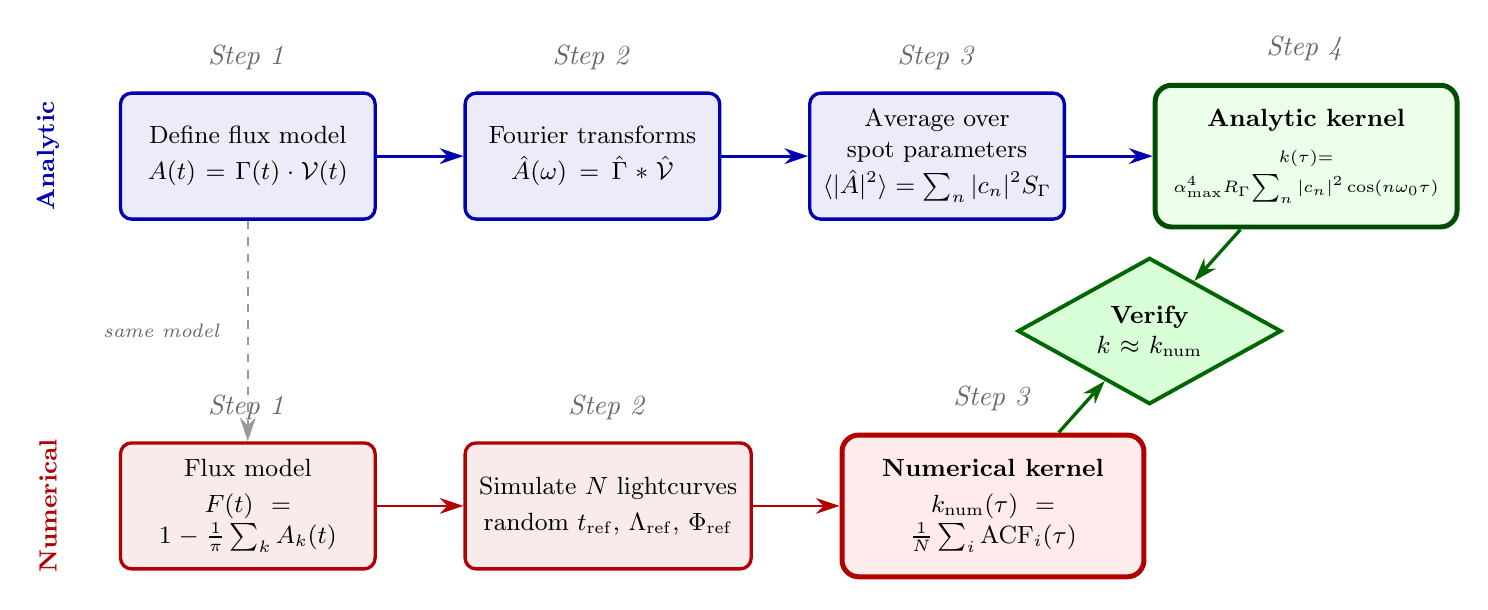
\begin{tikzpicture}[
    % Node styles
    box/.style={
        rectangle, rounded corners=4pt, draw=#1, fill=#1!8,
        line width=1.2pt, text width=3.0cm, minimum height=1.6cm,
        align=center, font=\small
    },
    box/.default=black,
    analytic/.style={box=blue!70!black},
    numerical/.style={box=red!70!black},
    result/.style={
        rectangle, rounded corners=6pt, draw=black!70!green, fill=green!8,
        line width=1.8pt, text width=3.6cm, minimum height=1.8cm,
        align=center, font=\small\bfseries
    },
    verify/.style={
        diamond, draw=black!60!green, fill=green!15,
        line width=1.4pt, text width=1.8cm,
        align=center, font=\small\bfseries, inner sep=2pt,
        aspect=1.8
    },
    arr/.style={
        -{Stealth[length=3mm, width=2mm]}, line width=1.0pt, color=#1
    },
    arr/.default=black!60,
    label/.style={font=\normalsize, text=black!60, align=center},
    rowlabel/.style={font=\small\bfseries\scshape, rotate=90, anchor=center},
]

% ═══════════════════════════════════════════════════════════════
% Row 1: Analytic derivation (top)
% ═══════════════════════════════════════════════════════════════

\node[analytic] (A1) {
    Define flux model\\[2pt]
    $A(t) = \Gamma(t) \cdot \mathcal{V}(t)$
};

\node[analytic, right=1.1cm of A1] (A2) {
    Fourier transforms\\[2pt]
    $\hat{A}(\omega) = \hat{\Gamma} \ast \hat{\mathcal{V}}$
};

\node[analytic, right=1.1cm of A2] (A3) {
    Average over\\spot parameters\\[2pt]
    $\langle|\hat{A}|^2\rangle = \sum_n |c_n|^2 S_\Gamma$
};

\node[result, right=1.1cm of A3] (A4) {
    Analytic kernel\\[2pt]
    $\scriptstyle k(\tau) = \alpha_{\max}^4 R_\Gamma \!\sum_n |c_n|^2 \cos(n\omega_0\tau)$
};

% Arrows (analytic row)
\draw[arr=blue!70!black] (A1) -- (A2);
\draw[arr=blue!70!black] (A2) -- (A3);
\draw[arr=blue!70!black] (A3) -- (A4);

% Step labels
\node[label, above=0.15cm of A1] {\textit{Step 1}};
\node[label, above=0.15cm of A2] {\textit{Step 2}};
\node[label, above=0.15cm of A3] {\textit{Step 3}};
\node[label, above=0.15cm of A4] {\textit{Step 4}};

% Row label (centered vertically with the row)
\node[rowlabel, blue!70!black] at ($(A1.west)+(-0.9cm,0)$) {Analytic};

% ═══════════════════════════════════════════════════════════════
% Row 2: Numerical verification (bottom)
% ═══════════════════════════════════════════════════════════════

\node[numerical, below=2.8cm of A1] (N1) {
    Flux model\\[2pt]
    $F(t) = 1 - \frac{1}{\pi}\sum_k A_k(t)$
};

\node[numerical, right=1.1cm of N1, text width=3.4cm] (N2) {
    Simulate $N$ lightcurves\\[2pt]
    random $t_{\rm ref}$, $\Lambda_{\rm ref}$, $\Phi_{\rm ref}$
};

\node[result, right=1.1cm of N2, fill=red!8, draw=red!70!black] (N3) {
    Numerical kernel\\[2pt]
    $k_{\rm num}(\tau) = \frac{1}{N}\sum_i \mathrm{ACF}_i(\tau)$
};

% Arrows (numerical row)
\draw[arr=red!70!black] (N1) -- (N2);
\draw[arr=red!70!black] (N2) -- (N3);

% Step labels
\node[label, above=0.15cm of N1] {\textit{Step 1}};
\node[label, above=0.15cm of N2] {\textit{Step 2}};
\node[label, above=0.15cm of N3] {\textit{Step 3}};

% Row label (centered vertically with the row)
\node[rowlabel, red!70!black] at ($(N1.west)+(-0.9cm,0)$) {Numerical};

% ═══════════════════════════════════════════════════════════════
% Convergence / verification
% ═══════════════════════════════════════════════════════════════

% Place the verification node between analytic result and numerical result
\node[verify] (V) at ($(A4)!0.5!(N3)$) {
    Verify\\$k \approx k_{\rm num}$
};

\draw[arr=black!60!green, line width=1.2pt] (A4) -- (V);
\draw[arr=black!60!green, line width=1.2pt] (N3) -- (V);

% Shared starting point arrow
\draw[arr=black!40, dashed, line width=0.8pt]
    (A1.south) -- ++(0, -0.7cm) -| (N1.north);

\node[label, font=\scriptsize\itshape] at ($(A1.south)!0.5!(N1.north) + (-1.1cm, 0)$) {same model};

\end{tikzpicture}
\caption{Overview of the kernel derivation strategy. \textit{Top row (blue):} The analytic path derives $k(\tau)$ from the single-spot flux model $A(t) = \Gamma(t)\cdot\mathcal{V}(t)$ by (1) computing Fourier transforms of the envelope and visibility terms, (2) averaging the energy spectral density over random spot parameters ($t_{\rm ref}$, $\Lambda_{\rm ref}$, $\Phi_{\rm ref}$), and (3) applying the Wiener--Khinchin theorem. \textit{Bottom row (red):} The numerical path simulates $N$ lightcurves from the same flux model with randomly drawn spot parameters and estimates the kernel as the sample-averaged autocorrelation. \textit{Center (green):} The two paths converge, verifying the analytic kernel against the numerical estimate.}
\label{fig:overview}
\end{figure*}

% Requires: \usepackage{tikz} in the preamble

\usetikzlibrary{arrows.meta, positioning, calc, backgrounds, fit, shapes.geometric}

\begin{figure*}[ht!]
\centering
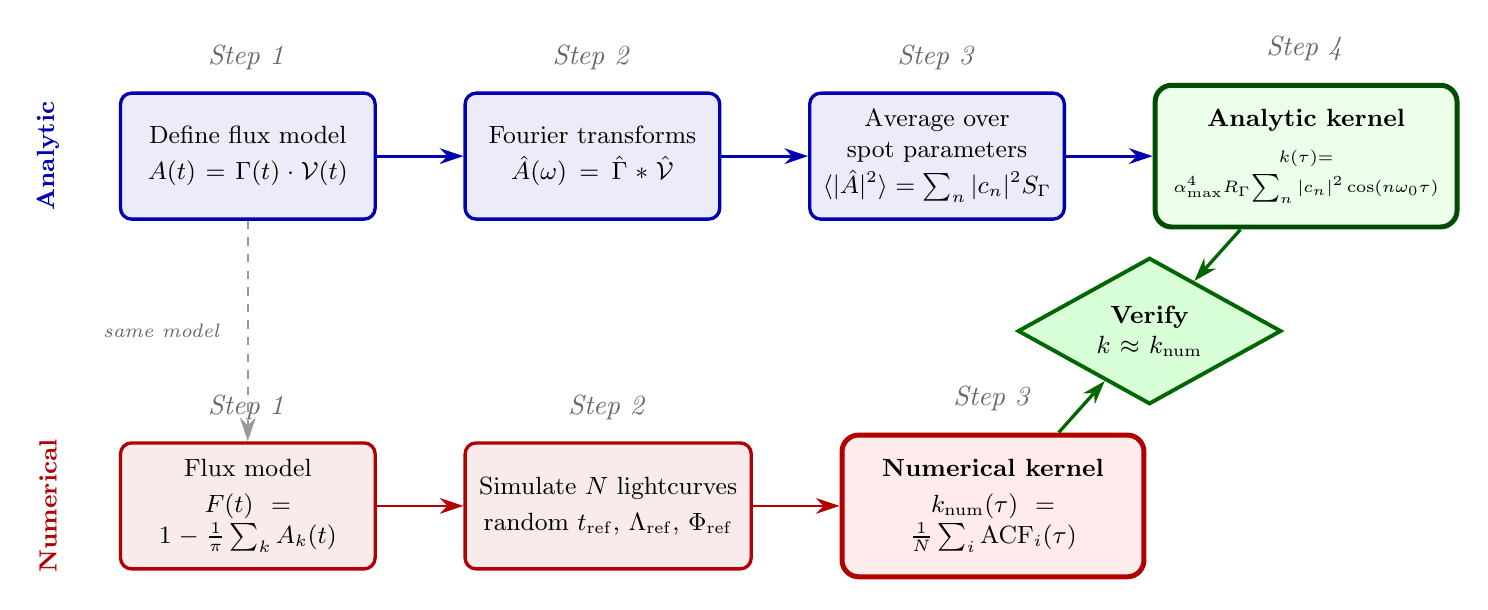
\begin{tikzpicture}[
    % Node styles
    box/.style={
        rectangle, rounded corners=4pt, draw=#1, fill=#1!8,
        line width=1.2pt, text width=3.0cm, minimum height=1.6cm,
        align=center, font=\small
    },
    box/.default=black,
    analytic/.style={box=blue!70!black},
    numerical/.style={box=red!70!black},
    result/.style={
        rectangle, rounded corners=6pt, draw=black!70!green, fill=green!8,
        line width=1.8pt, text width=3.6cm, minimum height=1.8cm,
        align=center, font=\small\bfseries
    },
    verify/.style={
        diamond, draw=black!60!green, fill=green!15,
        line width=1.4pt, text width=1.8cm,
        align=center, font=\small\bfseries, inner sep=2pt,
        aspect=1.8
    },
    arr/.style={
        -{Stealth[length=3mm, width=2mm]}, line width=1.0pt, color=#1
    },
    arr/.default=black!60,
    label/.style={font=\normalsize, text=black!60, align=center},
    rowlabel/.style={font=\small\bfseries\scshape, rotate=90, anchor=center},
]

% ═══════════════════════════════════════════════════════════════
% Row 1: Analytic derivation (top)
% ═══════════════════════════════════════════════════════════════

\node[analytic] (A1) {
    Define flux model\\[2pt]
    $A(t) = \Gamma(t) \cdot \mathcal{V}(t)$
};

\node[analytic, right=1.1cm of A1] (A2) {
    Fourier transforms\\[2pt]
    $\hat{A}(\omega) = \hat{\Gamma} \ast \hat{\mathcal{V}}$
};

\node[analytic, right=1.1cm of A2] (A3) {
    Average over\\spot parameters\\[2pt]
    $\langle|\hat{A}|^2\rangle = \sum_n |c_n|^2 S_\Gamma$
};

\node[result, right=1.1cm of A3] (A4) {
    Analytic kernel\\[2pt]
    $\scriptstyle k(\tau) = \alpha_{\max}^4 R_\Gamma \!\sum_n |c_n|^2 \cos(n\omega_0\tau)$
};

% Arrows (analytic row)
\draw[arr=blue!70!black] (A1) -- (A2);
\draw[arr=blue!70!black] (A2) -- (A3);
\draw[arr=blue!70!black] (A3) -- (A4);

% Step labels
\node[label, above=0.15cm of A1] {\textit{Step 1}};
\node[label, above=0.15cm of A2] {\textit{Step 2}};
\node[label, above=0.15cm of A3] {\textit{Step 3}};
\node[label, above=0.15cm of A4] {\textit{Step 4}};

% Row label (centered vertically with the row)
\node[rowlabel, blue!70!black] at ($(A1.west)+(-0.9cm,0)$) {Analytic};

% ═══════════════════════════════════════════════════════════════
% Row 2: Numerical verification (bottom)
% ═══════════════════════════════════════════════════════════════

\node[numerical, below=2.8cm of A1] (N1) {
    Flux model\\[2pt]
    $F(t) = 1 - \frac{1}{\pi}\sum_k A_k(t)$
};

\node[numerical, right=1.1cm of N1, text width=3.4cm] (N2) {
    Simulate $N$ lightcurves\\[2pt]
    random $t_{\rm ref}$, $\Lambda_{\rm ref}$, $\Phi_{\rm ref}$
};

\node[result, right=1.1cm of N2, fill=red!8, draw=red!70!black] (N3) {
    Numerical kernel\\[2pt]
    $k_{\rm num}(\tau) = \frac{1}{N}\sum_i \mathrm{ACF}_i(\tau)$
};

% Arrows (numerical row)
\draw[arr=red!70!black] (N1) -- (N2);
\draw[arr=red!70!black] (N2) -- (N3);

% Step labels
\node[label, above=0.15cm of N1] {\textit{Step 1}};
\node[label, above=0.15cm of N2] {\textit{Step 2}};
\node[label, above=0.15cm of N3] {\textit{Step 3}};

% Row label (centered vertically with the row)
\node[rowlabel, red!70!black] at ($(N1.west)+(-0.9cm,0)$) {Numerical};

% ═══════════════════════════════════════════════════════════════
% Convergence / verification
% ═══════════════════════════════════════════════════════════════

% Place the verification node between analytic result and numerical result
\node[verify] (V) at ($(A4)!0.5!(N3)$) {
    Verify\\$k \approx k_{\rm num}$
};

\draw[arr=black!60!green, line width=1.2pt] (A4) -- (V);
\draw[arr=black!60!green, line width=1.2pt] (N3) -- (V);

% Shared starting point arrow
\draw[arr=black!40, dashed, line width=0.8pt]
    (A1.south) -- ++(0, -0.7cm) -| (N1.north);

\node[label, font=\scriptsize\itshape] at ($(A1.south)!0.5!(N1.north) + (-1.1cm, 0)$) {same model};

\end{tikzpicture}
\caption{Overview of the kernel derivation strategy. \textit{Top row (blue):} The analytic path derives $k(\tau)$ from the single-spot flux model $A(t) = \Gamma(t)\cdot\mathcal{V}(t)$ by (1) computing Fourier transforms of the envelope and visibility terms, (2) averaging the energy spectral density over random spot parameters ($t_{\rm ref}$, $\Lambda_{\rm ref}$, $\Phi_{\rm ref}$), and (3) applying the Wiener--Khinchin theorem. \textit{Bottom row (red):} The numerical path simulates $N$ lightcurves from the same flux model with randomly drawn spot parameters and estimates the kernel as the sample-averaged autocorrelation. \textit{Center (green):} The two paths converge, verifying the analytic kernel against the numerical estimate.}
\label{fig:overview}
\end{figure*}

% Requires: \usepackage{tikz} in the preamble

\usetikzlibrary{arrows.meta, positioning, calc, backgrounds, fit, shapes.geometric}

\begin{figure*}[ht!]
\centering
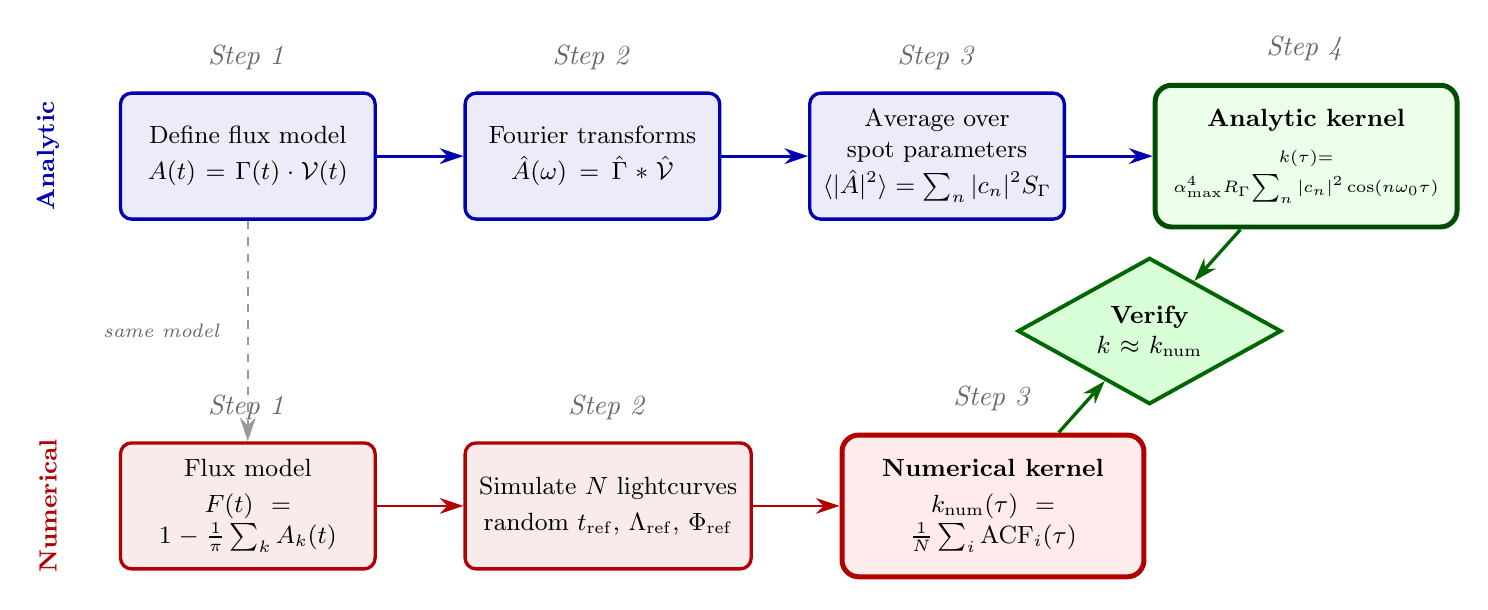
\begin{tikzpicture}[
    % Node styles
    box/.style={
        rectangle, rounded corners=4pt, draw=#1, fill=#1!8,
        line width=1.2pt, text width=3.0cm, minimum height=1.6cm,
        align=center, font=\small
    },
    box/.default=black,
    analytic/.style={box=blue!70!black},
    numerical/.style={box=red!70!black},
    result/.style={
        rectangle, rounded corners=6pt, draw=black!70!green, fill=green!8,
        line width=1.8pt, text width=3.6cm, minimum height=1.8cm,
        align=center, font=\small\bfseries
    },
    verify/.style={
        diamond, draw=black!60!green, fill=green!15,
        line width=1.4pt, text width=1.8cm,
        align=center, font=\small\bfseries, inner sep=2pt,
        aspect=1.8
    },
    arr/.style={
        -{Stealth[length=3mm, width=2mm]}, line width=1.0pt, color=#1
    },
    arr/.default=black!60,
    label/.style={font=\normalsize, text=black!60, align=center},
    rowlabel/.style={font=\small\bfseries\scshape, rotate=90, anchor=center},
]

% ═══════════════════════════════════════════════════════════════
% Row 1: Analytic derivation (top)
% ═══════════════════════════════════════════════════════════════

\node[analytic] (A1) {
    Define flux model\\[2pt]
    $A(t) = \Gamma(t) \cdot \mathcal{V}(t)$
};

\node[analytic, right=1.1cm of A1] (A2) {
    Fourier transforms\\[2pt]
    $\hat{A}(\omega) = \hat{\Gamma} \ast \hat{\mathcal{V}}$
};

\node[analytic, right=1.1cm of A2] (A3) {
    Average over\\spot parameters\\[2pt]
    $\langle|\hat{A}|^2\rangle = \sum_n |c_n|^2 S_\Gamma$
};

\node[result, right=1.1cm of A3] (A4) {
    Analytic kernel\\[2pt]
    $\scriptstyle k(\tau) = \alpha_{\max}^4 R_\Gamma \!\sum_n |c_n|^2 \cos(n\omega_0\tau)$
};

% Arrows (analytic row)
\draw[arr=blue!70!black] (A1) -- (A2);
\draw[arr=blue!70!black] (A2) -- (A3);
\draw[arr=blue!70!black] (A3) -- (A4);

% Step labels
\node[label, above=0.15cm of A1] {\textit{Step 1}};
\node[label, above=0.15cm of A2] {\textit{Step 2}};
\node[label, above=0.15cm of A3] {\textit{Step 3}};
\node[label, above=0.15cm of A4] {\textit{Step 4}};

% Row label (centered vertically with the row)
\node[rowlabel, blue!70!black] at ($(A1.west)+(-0.9cm,0)$) {Analytic};

% ═══════════════════════════════════════════════════════════════
% Row 2: Numerical verification (bottom)
% ═══════════════════════════════════════════════════════════════

\node[numerical, below=2.8cm of A1] (N1) {
    Flux model\\[2pt]
    $F(t) = 1 - \frac{1}{\pi}\sum_k A_k(t)$
};

\node[numerical, right=1.1cm of N1, text width=3.4cm] (N2) {
    Simulate $N$ lightcurves\\[2pt]
    random $t_{\rm ref}$, $\Lambda_{\rm ref}$, $\Phi_{\rm ref}$
};

\node[result, right=1.1cm of N2, fill=red!8, draw=red!70!black] (N3) {
    Numerical kernel\\[2pt]
    $k_{\rm num}(\tau) = \frac{1}{N}\sum_i \mathrm{ACF}_i(\tau)$
};

% Arrows (numerical row)
\draw[arr=red!70!black] (N1) -- (N2);
\draw[arr=red!70!black] (N2) -- (N3);

% Step labels
\node[label, above=0.15cm of N1] {\textit{Step 1}};
\node[label, above=0.15cm of N2] {\textit{Step 2}};
\node[label, above=0.15cm of N3] {\textit{Step 3}};

% Row label (centered vertically with the row)
\node[rowlabel, red!70!black] at ($(N1.west)+(-0.9cm,0)$) {Numerical};

% ═══════════════════════════════════════════════════════════════
% Convergence / verification
% ═══════════════════════════════════════════════════════════════

% Place the verification node between analytic result and numerical result
\node[verify] (V) at ($(A4)!0.5!(N3)$) {
    Verify\\$k \approx k_{\rm num}$
};

\draw[arr=black!60!green, line width=1.2pt] (A4) -- (V);
\draw[arr=black!60!green, line width=1.2pt] (N3) -- (V);

% Shared starting point arrow
\draw[arr=black!40, dashed, line width=0.8pt]
    (A1.south) -- ++(0, -0.7cm) -| (N1.north);

\node[label, font=\scriptsize\itshape] at ($(A1.south)!0.5!(N1.north) + (-1.1cm, 0)$) {same model};

\end{tikzpicture}
\caption{Overview of the kernel derivation strategy. \textit{Top row (blue):} The analytic path derives $k(\tau)$ from the single-spot flux model $A(t) = \Gamma(t)\cdot\mathcal{V}(t)$ by (1) computing Fourier transforms of the envelope and visibility terms, (2) averaging the energy spectral density over random spot parameters ($t_{\rm ref}$, $\Lambda_{\rm ref}$, $\Phi_{\rm ref}$), and (3) applying the Wiener--Khinchin theorem. \textit{Bottom row (red):} The numerical path simulates $N$ lightcurves from the same flux model with randomly drawn spot parameters and estimates the kernel as the sample-averaged autocorrelation. \textit{Center (green):} The two paths converge, verifying the analytic kernel against the numerical estimate.}
\label{fig:overview}
\end{figure*}

% Requires: \usepackage{tikz} in the preamble

\usetikzlibrary{arrows.meta, positioning, calc, backgrounds, fit, shapes.geometric}

\begin{figure*}[ht!]
\centering
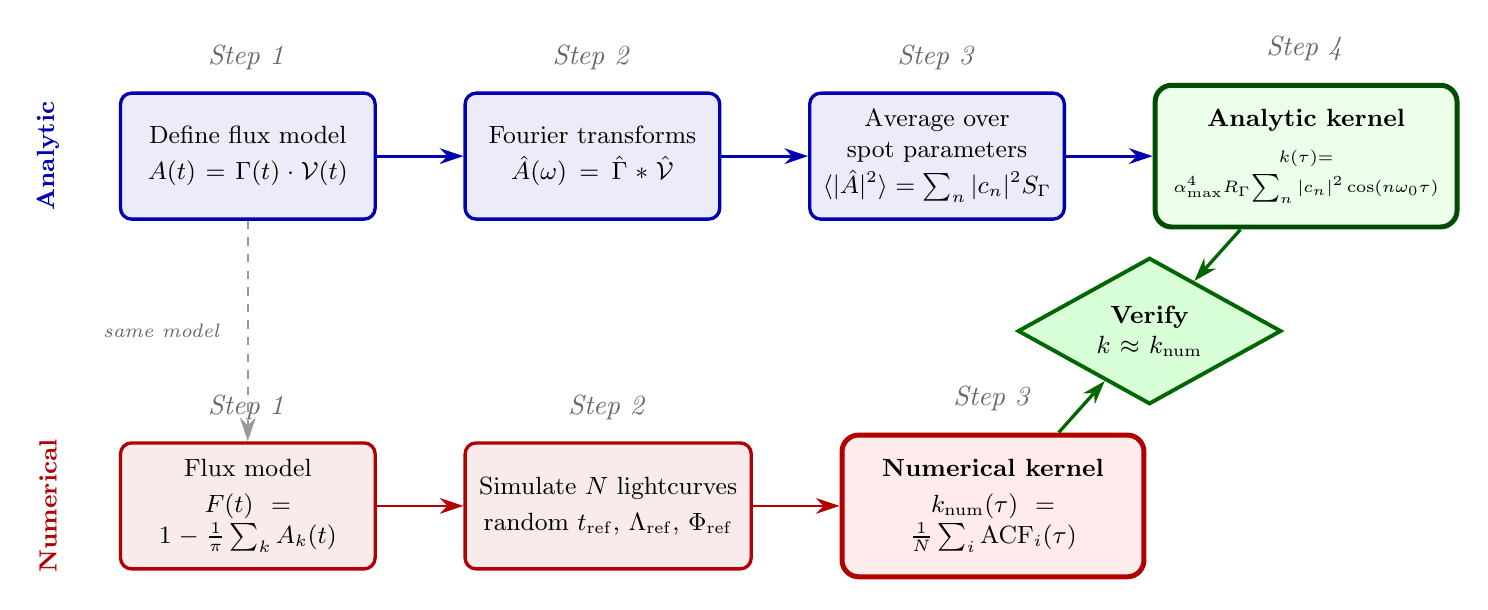
\begin{tikzpicture}[
    % Node styles
    box/.style={
        rectangle, rounded corners=4pt, draw=#1, fill=#1!8,
        line width=1.2pt, text width=3.0cm, minimum height=1.6cm,
        align=center, font=\small
    },
    box/.default=black,
    analytic/.style={box=blue!70!black},
    numerical/.style={box=red!70!black},
    result/.style={
        rectangle, rounded corners=6pt, draw=black!70!green, fill=green!8,
        line width=1.8pt, text width=3.6cm, minimum height=1.8cm,
        align=center, font=\small\bfseries
    },
    verify/.style={
        diamond, draw=black!60!green, fill=green!15,
        line width=1.4pt, text width=1.8cm,
        align=center, font=\small\bfseries, inner sep=2pt,
        aspect=1.8
    },
    arr/.style={
        -{Stealth[length=3mm, width=2mm]}, line width=1.0pt, color=#1
    },
    arr/.default=black!60,
    label/.style={font=\normalsize, text=black!60, align=center},
    rowlabel/.style={font=\small\bfseries\scshape, rotate=90, anchor=center},
]

% ═══════════════════════════════════════════════════════════════
% Row 1: Analytic derivation (top)
% ═══════════════════════════════════════════════════════════════

\node[analytic] (A1) {
    Define flux model\\[2pt]
    $A(t) = \Gamma(t) \cdot \mathcal{V}(t)$
};

\node[analytic, right=1.1cm of A1] (A2) {
    Fourier transforms\\[2pt]
    $\hat{A}(\omega) = \hat{\Gamma} \ast \hat{\mathcal{V}}$
};

\node[analytic, right=1.1cm of A2] (A3) {
    Average over\\spot parameters\\[2pt]
    $\langle|\hat{A}|^2\rangle = \sum_n |c_n|^2 S_\Gamma$
};

\node[result, right=1.1cm of A3] (A4) {
    Analytic kernel\\[2pt]
    $\scriptstyle k(\tau) = \alpha_{\max}^4 R_\Gamma \!\sum_n |c_n|^2 \cos(n\omega_0\tau)$
};

% Arrows (analytic row)
\draw[arr=blue!70!black] (A1) -- (A2);
\draw[arr=blue!70!black] (A2) -- (A3);
\draw[arr=blue!70!black] (A3) -- (A4);

% Step labels
\node[label, above=0.15cm of A1] {\textit{Step 1}};
\node[label, above=0.15cm of A2] {\textit{Step 2}};
\node[label, above=0.15cm of A3] {\textit{Step 3}};
\node[label, above=0.15cm of A4] {\textit{Step 4}};

% Row label (centered vertically with the row)
\node[rowlabel, blue!70!black] at ($(A1.west)+(-0.9cm,0)$) {Analytic};

% ═══════════════════════════════════════════════════════════════
% Row 2: Numerical verification (bottom)
% ═══════════════════════════════════════════════════════════════

\node[numerical, below=2.8cm of A1] (N1) {
    Flux model\\[2pt]
    $F(t) = 1 - \frac{1}{\pi}\sum_k A_k(t)$
};

\node[numerical, right=1.1cm of N1, text width=3.4cm] (N2) {
    Simulate $N$ lightcurves\\[2pt]
    random $t_{\rm ref}$, $\Lambda_{\rm ref}$, $\Phi_{\rm ref}$
};

\node[result, right=1.1cm of N2, fill=red!8, draw=red!70!black] (N3) {
    Numerical kernel\\[2pt]
    $k_{\rm num}(\tau) = \frac{1}{N}\sum_i \mathrm{ACF}_i(\tau)$
};

% Arrows (numerical row)
\draw[arr=red!70!black] (N1) -- (N2);
\draw[arr=red!70!black] (N2) -- (N3);

% Step labels
\node[label, above=0.15cm of N1] {\textit{Step 1}};
\node[label, above=0.15cm of N2] {\textit{Step 2}};
\node[label, above=0.15cm of N3] {\textit{Step 3}};

% Row label (centered vertically with the row)
\node[rowlabel, red!70!black] at ($(N1.west)+(-0.9cm,0)$) {Numerical};

% ═══════════════════════════════════════════════════════════════
% Convergence / verification
% ═══════════════════════════════════════════════════════════════

% Place the verification node between analytic result and numerical result
\node[verify] (V) at ($(A4)!0.5!(N3)$) {
    Verify\\$k \approx k_{\rm num}$
};

\draw[arr=black!60!green, line width=1.2pt] (A4) -- (V);
\draw[arr=black!60!green, line width=1.2pt] (N3) -- (V);

% Shared starting point arrow
\draw[arr=black!40, dashed, line width=0.8pt]
    (A1.south) -- ++(0, -0.7cm) -| (N1.north);

\node[label, font=\scriptsize\itshape] at ($(A1.south)!0.5!(N1.north) + (-1.1cm, 0)$) {same model};

\end{tikzpicture}
\caption{Overview of the kernel derivation strategy. \textit{Top row (blue):} The analytic path derives $k(\tau)$ from the single-spot flux model $A(t) = \Gamma(t)\cdot\mathcal{V}(t)$ by (1) computing Fourier transforms of the envelope and visibility terms, (2) averaging the energy spectral density over random spot parameters ($t_{\rm ref}$, $\Lambda_{\rm ref}$, $\Phi_{\rm ref}$), and (3) applying the Wiener--Khinchin theorem. \textit{Bottom row (red):} The numerical path simulates $N$ lightcurves from the same flux model with randomly drawn spot parameters and estimates the kernel as the sample-averaged autocorrelation. \textit{Center (green):} The two paths converge, verifying the analytic kernel against the numerical estimate.}
\label{fig:overview}
\end{figure*}
